\documentclass[../AnalysisNoteJBuxton.tex]{subfiles}
\begin{document}

\subsection{Model: Lambda-Kaon}
\label{ModelLambdaKaon}

Talk about Lednicky model

\begin{figure}[h]
  \centering
  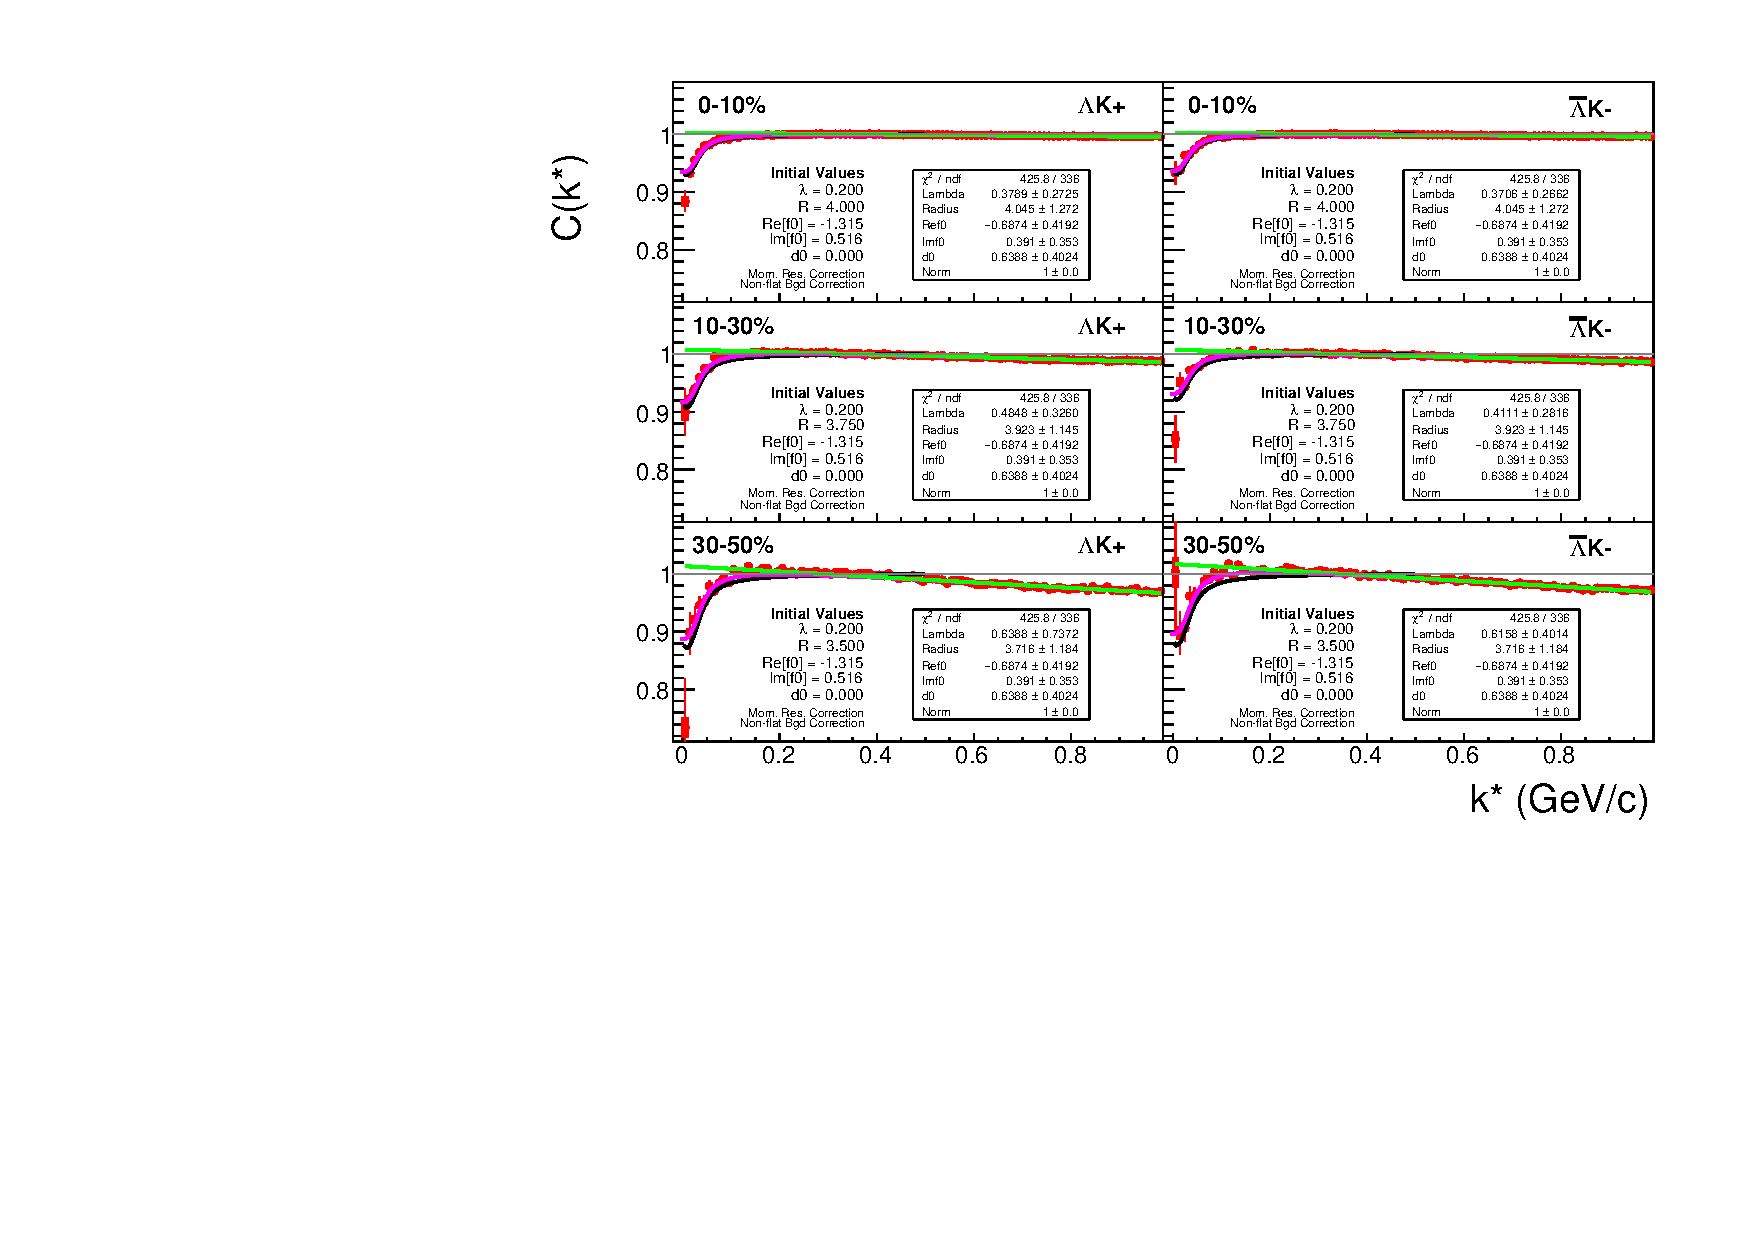
\includegraphics[width=\textwidth]{5_Fitting/Figures/canKStarCfwFitsLamKchPwConj_MomResCrctn_NonFlatBgdCrctn.pdf}
  \caption[$\Lambda$K$^{+}$($\bar{\Lambda}$K$^{-}$) Fits]{$\Lambda$K$^{+}$($\bar{\Lambda}$K$^{-}$) Fits}
  \label{fig:LamKchPwConjFits}
\end{figure}

\begin{figure}[h]
  \centering
  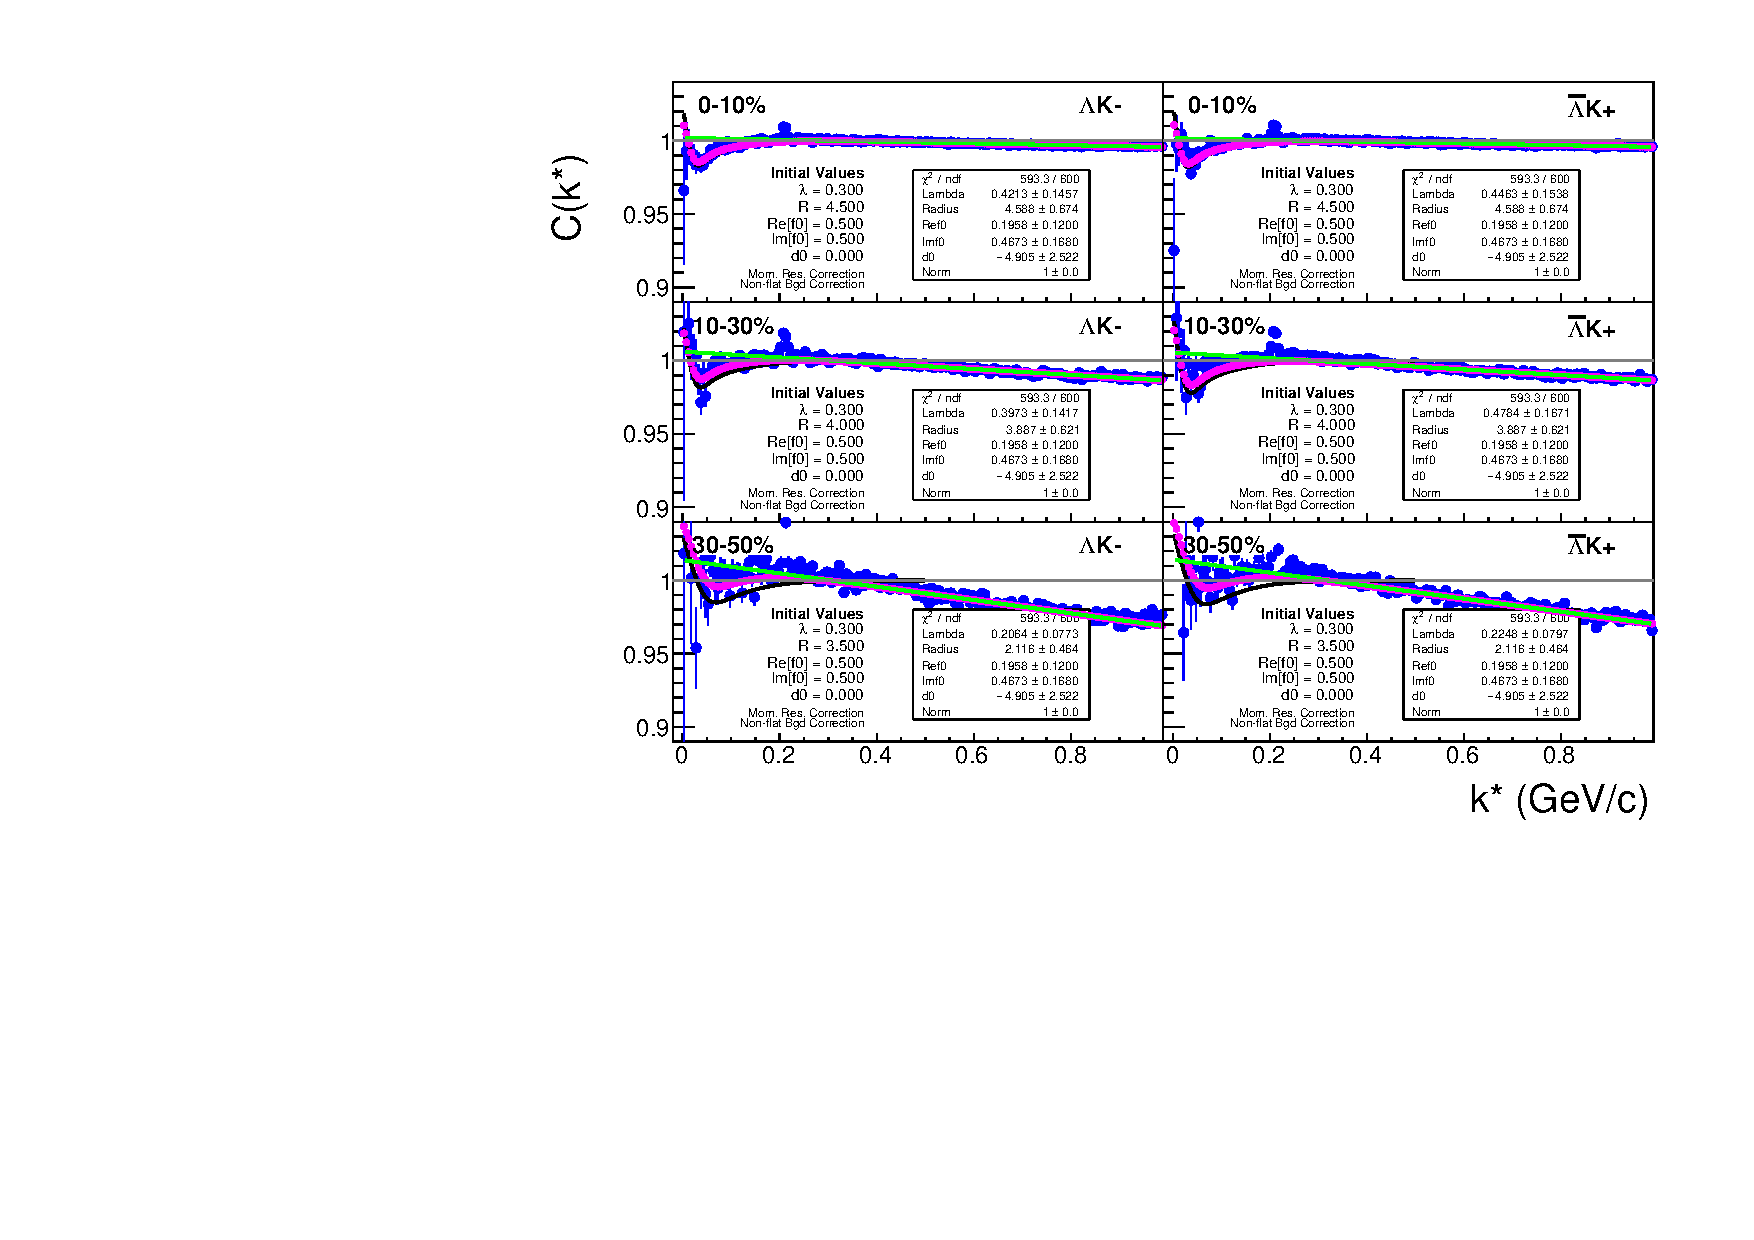
\includegraphics[width=\textwidth]{5_Fitting/Figures/canKStarCfwFitsLamKchMwConj_MomResCrctn_NonFlatBgdCrctn.pdf}
  \caption[$\Lambda$K$^{-}$($\bar{\Lambda}$K$^{+}$) Fits]{$\Lambda$K$^{-}$($\bar{\Lambda}$K$^{+}$) Fits}
  \label{fig:LamKchMwConjFits}
\end{figure}

\end{document}